\begin{taged}{自醒,家事}
  \section{2024-08-14-狼走千里吃肉}
\end{taged}

\begin{figure}[htbp]
    \centering
    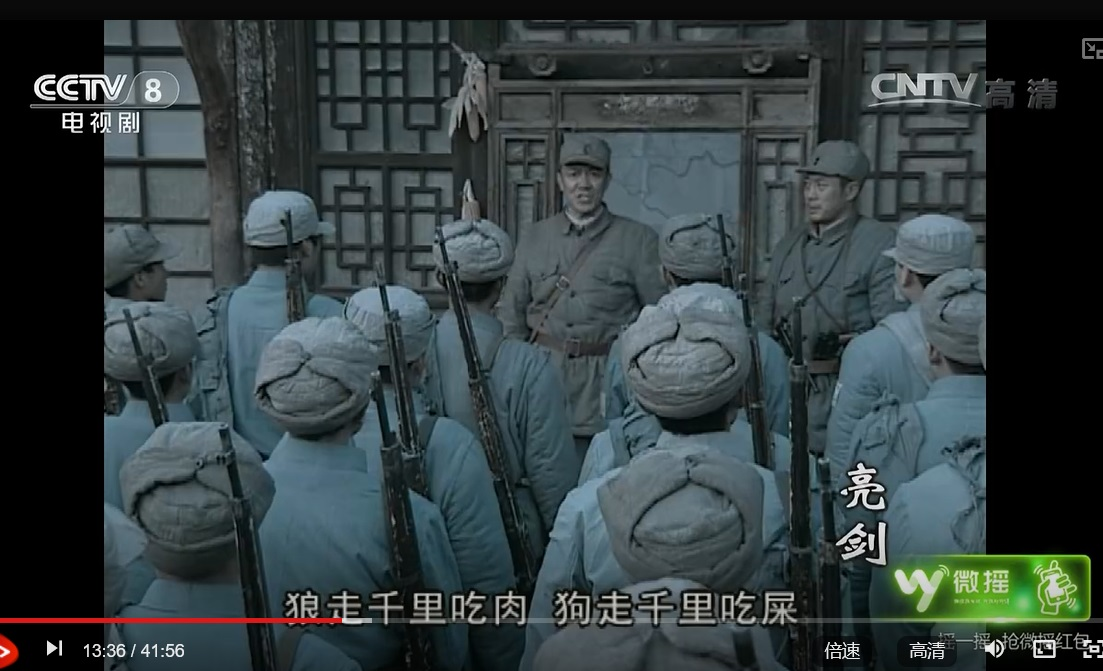
\includegraphics[width=10cm]{pic/狼走千里.jpg}
    \caption*{狼走千里吃肉\footnotemark}
\end{figure}
\footnotetext{2005 年\href{https://tv.cctv.com/2015/08/27/VIDE1440638297499214.shtml}{《亮剑》第二集},李云龙刚到独立团任团长时,给部下的讲话。}

"狼走千里吃肉,狗走千里吃屎。" 这话怎么理解?

\zhongdian{要么成为狼,练就吃肉的本领;要么成为狗,拥有吃屎的胃口。}




